% Drawing 161-6/01-1 -- folder 161-6, batch 01, archive page 3 (PDF page 4).
% Transcription: en marge gauche, au bas de la page, une figure : du point $u$, l'arc de grand cercle vers $x(u,v;\alpha)$ et celui vers $x(u,v';\alpha)$, l'angle $\theta$ entre eux marqué près de $u$ ; un trait épais joint $u$ au centre, d'où partent en tirets les rayons vers les deux points $x$, l'angle $\alpha$ marqué près du centre ; en bas, les vecteurs $v$, $v'$, $w$ issus du centre, un arc passant par leurs extrémités et l'angle $\theta$ entre $v$ et $v'$.
% Kind: spherical triangle from u with the vectors v, v', w. Method 2 (schematic redraw from the facsimile). Status: partial.
% Notes: Small ink figure in the left margin. From the point u, two arcs, to x(u,v;alpha) above and to x(u,v';alpha) at the left, both ending at the one point u; a small arc between them near u and the letter theta; a heavy stroke from u down to the centre; from the centre, dash-dotted radii to the two points x; alpha written near the centre, with two small arcs there. Below: three strokes from the centre to v, v' and w (arrowheads at v and w), an arc through the three ends, theta between v and v' with its small arc. All strokes from the centre start at one computed point. Still differs: the small arcs marking alpha are a reading of a few crowded strokes (he hatches a small fan there); the dash-dotted radius to x(u,v;alpha) is visible only in its upper part on the page and is drawn whole. The transcription's note has theta « près des sommets »: one theta near u and one below between v and v' are seen. Redrawn 2026-11-10 (issue 128): to check again. 2026-11-13, Claude Opus 5.5, issue 147, overlay check: not compiled (no TeX in the session); the TikZ was rasterised by a local interpreter and laid over the scan rendered at 400 dpi. Nothing changed. The strokes, arcs and points lie on their ink to within about one unit at the scale of the figure; it stays partial for the reading of the crowded small arcs and of the dash-dotted radius named above.
% Coordinates: 1 unit = 1 mm = 1/100 of the crop width (bbox in page fractions: [0.11, 0.715, 0.27, 0.835]).
% Redrawn by Claude (claude-fable-5-2), issue #128, 2026-11-10; not checked by a human; not compiled (no TeX in the session); overlay-checked on the scan by Claude Opus 5.5, issue #147, 2026-11-13, not compiled (no TeX in the session).
% Rights: reproduces part of the work -- behind RENDER_TRANSCRIPTS, never published by itself.
\documentclass[tikz,border=3pt]{standalone}
\usepackage{amsmath,amssymb}
\usetikzlibrary{patterns,arrows.meta}
\tikzset{pencil/.style={black!45}, struck/.style={black!35}, mpt/.style={circle,draw,inner sep=1.3pt}, pt/.style={circle,fill,inner sep=0.9pt}, opt/.style={circle,draw,fill=white,inner sep=1.1pt}}
\begin{document}
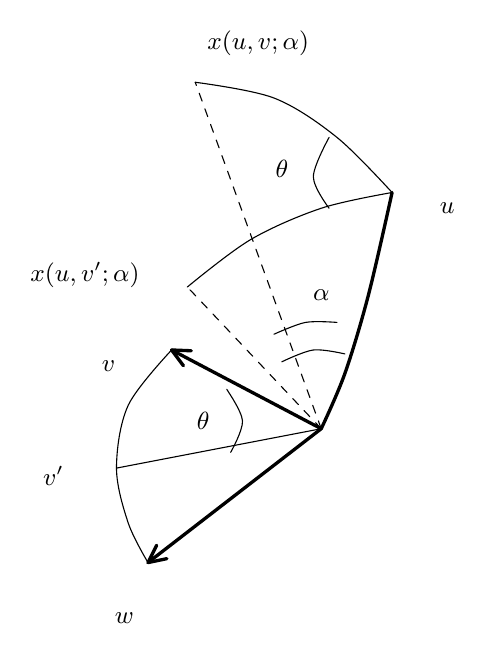
\begin{tikzpicture}[x=1mm,y=1mm,line cap=round,line join=round,font=\scriptsize]
\draw plot[smooth, tension=0.55] coordinates {(40,-23) (50,-25) (58,-30) (65,-37)};
\draw plot[smooth, tension=0.55] coordinates {(39,-49) (47,-43) (56,-39) (65,-37)};
\draw plot[smooth, tension=0.55] coordinates {(57,-30) (55,-35) (57,-39)};
\node[inner sep=1pt] at (51,-34) {\small $\theta$};
\draw[very thick] plot[smooth, tension=0.55] coordinates {(65,-37) (62,-50) (59,-60) (56,-67)};
\draw[dashed] (56,-67) -- (40,-23);
\draw[dashed] (56,-67) -- (39,-49);
\node[inner sep=1pt] at (56,-50) {\small $\alpha$};
\draw plot[smooth, tension=0.55] coordinates {(50,-55) (54,-53.5) (58,-53.5)};
\draw plot[smooth, tension=0.55] coordinates {(51,-58.5) (55,-57) (59,-57.5)};
\draw[very thick] (56,-67) -- (37,-57);
\draw[very thick] (38.5,-59) -- (37,-57) -- (39.5,-57.1);
\draw (56,-67) -- (30,-72);
\draw[very thick] (56,-67) -- (34,-84);
\draw[very thick] (36.4,-83.5) -- (34,-84) -- (35.1,-81.8);
\draw plot[smooth, tension=0.55] coordinates {(37,-57) (31.5,-64) (30,-72) (31.5,-79) (34,-84)};
\draw plot[smooth, tension=0.55] coordinates {(44,-62) (46,-66) (44.5,-70)};
\node[inner sep=1pt] at (41,-66) {\small $\theta$};
\node[inner sep=1pt] at (72,-39) {\small $u$};
\node[inner sep=1pt] at (48,-18) {\small $x(u,v;\alpha)$};
\node[inner sep=1pt] at (26,-47.5) {\small $x(u,v';\alpha)$};
\node[inner sep=1pt] at (29,-59) {\small $v$};
\node[inner sep=1pt] at (22,-73) {\small $v'$};
\node[inner sep=1pt] at (31,-91) {\small $w$};
\end{tikzpicture}
\end{document}
